\PassOptionsToPackage{unicode=true}{hyperref} % options for packages loaded elsewhere
\PassOptionsToPackage{hyphens}{url}
%
\documentclass[]{article}
\usepackage{lmodern}
\usepackage{amssymb,amsmath}
\usepackage{ifxetex,ifluatex}
\usepackage{fixltx2e} % provides \textsubscript
\ifnum 0\ifxetex 1\fi\ifluatex 1\fi=0 % if pdftex
  \usepackage[T1]{fontenc}
  \usepackage[utf8]{inputenc}
  \usepackage{textcomp} % provides euro and other symbols
\else % if luatex or xelatex
  \usepackage{unicode-math}
  \defaultfontfeatures{Ligatures=TeX,Scale=MatchLowercase}
\fi
% use upquote if available, for straight quotes in verbatim environments
\IfFileExists{upquote.sty}{\usepackage{upquote}}{}
% use microtype if available
\IfFileExists{microtype.sty}{%
\usepackage[]{microtype}
\UseMicrotypeSet[protrusion]{basicmath} % disable protrusion for tt fonts
}{}
\IfFileExists{parskip.sty}{%
\usepackage{parskip}
}{% else
\setlength{\parindent}{0pt}
\setlength{\parskip}{6pt plus 2pt minus 1pt}
}
\usepackage{hyperref}
\hypersetup{
            pdfborder={0 0 0},
            breaklinks=true}
\urlstyle{same}  % don't use monospace font for urls
\usepackage{longtable,booktabs}
% Fix footnotes in tables (requires footnote package)
\IfFileExists{footnote.sty}{\usepackage{footnote}\makesavenoteenv{longtable}}{}
\usepackage{graphicx,grffile}
\makeatletter
\def\maxwidth{\ifdim\Gin@nat@width>\linewidth\linewidth\else\Gin@nat@width\fi}
\def\maxheight{\ifdim\Gin@nat@height>\textheight\textheight\else\Gin@nat@height\fi}
\makeatother
% Scale images if necessary, so that they will not overflow the page
% margins by default, and it is still possible to overwrite the defaults
% using explicit options in \includegraphics[width, height, ...]{}
\setkeys{Gin}{width=\maxwidth,height=\maxheight,keepaspectratio}
\setlength{\emergencystretch}{3em}  % prevent overfull lines
\providecommand{\tightlist}{%
  \setlength{\itemsep}{0pt}\setlength{\parskip}{0pt}}
\setcounter{secnumdepth}{0}
% Redefines (sub)paragraphs to behave more like sections
\ifx\paragraph\undefined\else
\let\oldparagraph\paragraph
\renewcommand{\paragraph}[1]{\oldparagraph{#1}\mbox{}}
\fi
\ifx\subparagraph\undefined\else
\let\oldsubparagraph\subparagraph
\renewcommand{\subparagraph}[1]{\oldsubparagraph{#1}\mbox{}}
\fi

% set default figure placement to htbp
\makeatletter
\def\fps@figure{htbp}
\makeatother


\date{}

\begin{document}

\hypertarget{proyecciuxf3n-gauss-kruxfcger}{%
\subsection{PROYECCIÓN
GAUSS-KRÜGER}\label{proyecciuxf3n-gauss-kruxfcger}}

La teoría de la proyección conforme del elipsoide terrestre es
establecida por primera vez por el matemático Johann Karl Friedrich
Gauss (1777-1855) entre los años 1816 y 1827.

En el año 1821, Gauss aplicó su proyección en trabajos geodésicos en el
estado de Hannover.

En este sistema la superficie intermedia de proyección en un cilindro
tangente a la largo del meridiano central de la región que se quiere
representar; es apropiado para territorios cuya dirección de máxima
amplitud es en el sentido de las latitudes.

Las deformaciones dependen solamente del apartamiento del meridiano
central y son simétricas respecto del mismo.

Cuando se trata de representar territorios muy extendidos en el sentido
de las longitudes, se presentarán deformaciones importantes en los
puntos más alejados del meridiano central, que podrían exceder una
tolerancia prefijada.

Para resolver este problema, se divide el territorio en husos o fajas
meridianas de ancho tal que las mayores deformaciones no sobrepasen un
valor establecido. Los husos son sistemas de coordenadas independientes;
para lograr la vinculación de ellos se establecen zonas de superposición
en los límites de los mismos, donde se calculan las coordenadas en ambos
sistemas.

El geodesta L. Krüger del Instituto Geodésico de Postdam, introdujo en
1912 el empleo de las fajas meridianas y desde allí se generalizó el
nombre de la proyección.

Esta proyección busca fórmulas que den la transformación conforme de
puntos del elipsoide en puntos del plano.

Los puntos del elipsoide están caracterizados por sus coordenadas
geográficas latitud y longitud, y los puntos del plano por sus
coordenadas planas rectangulares X e Y. Se trata de establecer una
relación funcional entre el sistema elipsóidico y el plano de manera tal
que la representación sea conforme.

Esta transformación se lleva a cabo mediante una función de variable
compleja e imponiendo ciertas condiciones previas.

La imagen del meridiano central de la faja es el eje X, tomándolo con
sentido positivo hacia el norte.

Las magnitudes lineales sobre el meridiano central aparecen sin
deformación.

\hypertarget{proyecciuxf3n-gauss-kruxfcger.}{%
\subsubsection{PROYECCIÓN
GAUSS-KRÜGER.}\label{proyecciuxf3n-gauss-kruxfcger.}}

Dados dos puntos sobre el elipsoide infinitamente próximos (figura
IX.2), ambos vienen caracterizados por sus coordenadas geográficas
latitud y longitud. Teniendo en cuenta que ambos puntos son
infinitamente próximos, se puede considerar que la parcela elipsóidica
que abarcan no tienen curvatura, es decir que es un plano que se
denominará ``z'', es decir que la superficie elemental
\[\left(d\varphi,d\lambda \right)\] se supone plana.

Ambos puntos tienen su imagen plana, cuyas posiciones se caracterizan
por sus coordenadas planas ortogonales X e Y en la carta, que se
denominará plano de las ``u''.

Se trata de establecer la relación funcional entre la superficie
elipsóidica elemental con la correspondiente superficie plana, con la
condición que la representación sea conforme. De acuerdo con lo
anteriormente expuesto se hace uso de la funciones de variable compleja
porque ellas satisfacen dicha condición.

Se forman para cada plano las variables complejas:

\[z=\varphi + i \lambda\]

\[u=X+iY\] Ambas variables están ligadas por la función de variable
compleja:

\[u=f\left(z\right)\]

O sea:

\[X+iY=f\left(\varphi +\mathit{i\lambda
}\right)\] (X.7)

Formando la variable compleja \[\varphi +i\lambda \] no se ha elegido la
misma unidad lineal para la parte real y la parte imaginaria de la
variable. Si se incrementan en 1'' por ejemplo la latitud y longitud, el
arco de meridiano es siempre el mismo para cualquier latitud, no así el
arco de paralelo que disminuye a medida que la longitud aumenta.

Los arcos de meridiano y paralelo en el elipsoide son respectivamente:

\[dm=M\cdot d\varphi \] \[dp=N\cdot \text{cos}\left(\varphi
\right)\cdot d\lambda \] En la esfera:

\[dm=R\cdot d\varphi \] \[dp=R\cdot \text{cos}\left(\varphi
\right)\cdot d\lambda \] Por lo tanto el arco de paralelo disminuye de
acuerdo con el coseno de la latitud. Por ejemplo 1'' en el ecuador y a
60 de latitud le corresponden los siguientes arcos de meridiano y
paralelo:

\(dm\left(0{}^{\circ}\right)=\text{30}m\)

\(dp\left(0{}^{\circ}\right)=\text{30}m\)

\(dm\left(\text{60}{}^{\circ}\right)=\text{30}m\)

\(dp\left(\text{50}{}^{\circ}\right)=\text{15}m\)

Es decir, que sobre la superficie elipsóidica considerada plana, no se
tienen cuadrados elementales sino rectángulos elementales, por no
producir el mismo incremento lineal sobre el elipsoide, incrementos
iguales en latitud y longitud. Si:

\[d\varphi =d\lambda \] Las unidades lineales en el sentido de la
latitud y la longitud están en la relación:

\[\frac{dp}{dm}=\frac{M}{N\cdot \text{cos}\left(\varphi \right)}\]

Para igualar los arcos de meridiano y paralelo se sustituye la latitud
`` \$\emph{φ} \$'' por una nueva variable ``q'' llamada latitud
isométrica, contada también a partir del ecuador de manera que el
elemento de meridiano se exprese:

\[M\cdot d\varphi =N\cdot \text{cos}\left(\varphi \right)\cdot
dq\] Porque se desea que para iguales incrementos de latitud isométrica
y longitud:

\[dq=d\lambda \] Se produzcan iguales incrementos lineales sobre
meridianos y paralelos. Por lo tanto:

\[dq=\frac{M\cdot d\varphi }{N\cdot
\text{cos}\left(\varphi \right)}\] (X.8)

En el caso de una esfera sonde M=N=R se tiene que:

\[dq=\frac{\mathit{d\varphi
}}{\text{cos}\left(\varphi \right)}\] (X.8')

Si por ejemplo \[dq=\mathit{d\lambda
}=1\text{{\textquotesingle}{\textquotesingle}}\], en la latitud de 60 se
tiene que:

\[dm=R\cdot d\varphi =R\cdot
\text{cos}\left(\varphi \right)\cdot
dq=\text{15}m\] \[dm=R\cdot d\varphi =R\cdot
\text{cos}\left(\varphi \right)\cdot
dq=\text{15}m\] Integrando las (X.8) y (X.8'):

\[q=\text{ln}\left[tg\left(\text{45}\text{{\textdegree}+}\frac{\varphi
}{2}\right)\right]-\frac{e}{2}\cdot \text{ln}\left(\frac{1-e\cdot
sen\left(\varphi \right)}{1+e\cdot
sen\left(\varphi \right)}\right)\]
\[q=\text{ln}\left[tg\left(\text{45}\text{{\textdegree}+}\frac{\varphi
}{2}\right)\right]-\frac{e}{2}\cdot \text{ln}\left(\frac{1-e\cdot
sen\left(\varphi \right)}{1+e\cdot
sen\left(\varphi \right)}\right)\] Haciendo el cambio de variable en la
ecuación (X.7) se tiene que:

\[X+iY=f\left(q+\mathit{i\lambda
}\right)\] (X.9)

En esta proyección no se busca la representación del elipsoide entero,
sino de una faja comprendida entre dos meridianos no muy distanciados.
Teóricamente se podría representar el elipsoide entero en esta forma,
pero serían inevitables grandes dilataciones lineales a medida que los
puntos se apartan del meridiano central.

El origen de las longitudes no es el meridiano de Greenwich sino el
meridiano central de la faja que se pretende representar, de manera que
se efectúa otro cambio de variable ya que las longitudes se cuentan a
partir del meridiano central, positiva al este y negativa al oeste del
mismo, longitud que se denominará ``l'', tal que:

\[l=\lambda -\lambda _{M\text{.}C\text{.}}\] Se forma entonces la
función de variable compleja:

\[X+iY=f\left(q+il\right)\] (X.10)

donde ``q'' y ``l'' caracterizan la situación de cualquier punto sobre
la faja del elipsoide, y que en X e Y son las coordenadas planas de la
representación de ese pinto en el plano de la proyección.

Para que esta proyección esté completamente determinada, se impone una
condición que exige que los puntos del meridiano central sean
representados sin deformación lineal.

Además la imagen rectificada del meridiano central es el eje de las X de
la representación y para el hemisferio sur de origen de coordenadas (0,
0) se encuentra en el polo sur.

La condición de que en el meridiano central no se deformen las
magnitudes lineales es la condición de tangencia del cilindro a lo largo
de tal meridiano.

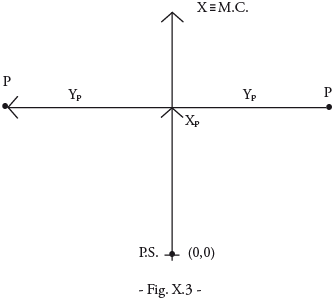
\includegraphics{repslatex-img81.png}

Por lo tanto los puntos situados sobre el meridiano central tienen
coordenadas:

\[l=0\] \[Y=0\] sobre el elipsoide y la carta, respectivamente.

La función (X.10) para dichos puntos se transforma en:

\[X=f\left(q\right)\] Los puntos del meridiano central están
representados por puntos en una recta, eje de las X, en tal forma que
sus distancias relativas son iguales en la proyección y en el elipsoide.

De lo anterior se deduce la naturaleza de la (X.11), que expresa el arco
de meridiano del polo sur al punto considerado, por la variable ``q'' la
que en cualquier momento se puede reemplazar por la variable
\[\varphi \].

La función que expresa tal magnitud, como se determinó en VIII.5 es:

\[S=\overset{{\varphi }}{\underset{{-\pi /2}}{\int }}{M\cdot
d\varphi }\] De modo que se tiene:

\[S=f\left(q\right)\] (X.12)

Para encontrar las coordenadas X e Y de puntos que no se encuentran
sobre el meridiano central, se desarrolla en serie de Taylor la función
de variable compleja (X.10) tomando como origen dicho meridiano y como
incremento la diferencia de longitud ``l''.

Se obtiene por lo tanto:

\[X+iY=f\left(q\right)+\frac{df\left(q\right)}{dq}\cdot
\left(il\right)+\frac{d^2f\left(q\right)}{dq^2}\cdot
{\frac{\left(il\right)^2}{2!}}+\frac{d^3f\left(q\right)}{dq^3}\cdot
{\frac{\left(il\right)}{3!}}^3+\text{.}\text{.}\text{.}\] O bien
teniendo en cuenta la (X.12):

\[X+iY=S+\frac{dS}{dq}\cdot
\left(il\right)+\frac{d^2S}{dq^2}\cdot
{\frac{\left(il\right)^2}{2!}}+\frac{d^3S}{dq^3}\cdot
{\frac{\left(il\right)}{3!}}^3+\text{.}\text{.}\text{.}\] Los términos
del desarrollo en serie pares son reales porque:

\[i^2=-1\] \[i^4=i^2\cdot i^2=\left(-1\right)\cdot \left(-1\right)=1\]
\[i^6=i^4\cdot i^2=1\cdot \left(-1\right)=-1\] Por lo tanto los términos
de derivadas pares corresponden a las X; los términos de derivadas
impares son imaginarios puros porque:

\[i^3=i^2\cdot i=-i\]
\[i^5=i^3\cdot i^2=\left(-i\right)\cdot \left(-1\right)=i\] Por lo tanto
corresponden a las Y. Es posible entonces separar las variables reales e
imaginarias:

\[X=S-\frac{d^2S}{dq^2}\cdot {\frac{l^2}{2}}+\frac{d^4S}{dq^4}\cdot {\frac{l}{\text{24}}}^4-\frac{d^6S}{dq^6}\cdot {\frac{l^6}{\text{720}}}+\text{.}\text{.}\text{.}\]

\[Y=\frac{dS}{dq}\cdot l-\frac{d^3S}{dq^3}\cdot {\frac{l}{6}}^3+\frac{d^5S}{dq^5}\cdot {\frac{l^5}{\text{120}}}-\text{.}\text{.}\text{.}\]
(X.13.b)

Se calculará el primer término de la serie:

\[\frac{dS}{dq}=\frac{dS}{\mathit{d\varphi
}}\cdot {\frac{d\varphi }{dq}}\] \[dS=M\cdot d\varphi \]
\[\frac{dS}{d\varphi }=M\] \[dq=\frac{M\cdot d\varphi }{N\cdot
\text{cos}\left(\varphi \right)}\] \[\frac{d\varphi }{dq}=\frac{N\cdot
\text{cos}\left[\varphi \right]}{M}\] Por lo tanto:

\[\frac{dS}{dq}=M\cdot {\frac{N\cdot \text{cos}\left(\varphi \right)}{M}}\]

\[\frac{dS}{dq}=N\cdot \text{cos}\left(\varphi \right)\]

Para hallar las sucesivas derivadas de ``S'' respecto de ``q'' se deriva
como función de función, primero respecto de la variable ``
\[\varphi \]'' y luego por ``q''. Llamando:

\[F^{II}=\frac{d^2S}{dq^2}=\frac{d}{d\varphi}\left(\frac{dS}{dq}\right)\frac{d\varphi}{dq}\]

\[\frac{d}{d\varphi}\left(\frac{dS}{dq}\right)=\frac{d}{d\varphi}\left[N\text{cos}\left(\varphi \right)\right]=\frac{dN}{d\varphi}\cdot \text{cos}\left(\varphi \right)-N\cdot sen\left(\varphi \right)\]

\[N=a\cdot \left[1-e^2\cdot sen^2\left(\varphi \right)\right]^{-1/2}\]

\[\frac{dN}{d\varphi }=a\cdot \left[1-e^2\cdot sen^2\left(\varphi \right)\right]^{-3/2}\cdot e^2\cdot sen\left(\varphi \right)\cdot \text{cos}\left(\varphi \right)=\frac{N\cdot e^2\cdot sen\left(\varphi \right)\cdot \text{cos}\left(\varphi \right)}{1-e^2\cdot sen^2\left(\varphi \right)}\]

\[\frac{d}{d\varphi}\left(\frac{dS}{dq}\right)=\left[\frac{N\cdot e^2\cdot sen\left(\varphi \right)\cdot \text{cos}\left(\varphi \right)}{1-e^2\cdot sen^2\left(\varphi \right)}\right]\cdot \text{cos}\left(\varphi \right)-N\cdot sen\left(\varphi \right)=\]

\[=\frac{N\cdot e^2\cdot sen\left(\varphi \right)\cdot \text{cos}^2\left(\varphi \right)-N\cdot sen\left(\varphi \right)\cdot \left[1-e^2\cdot sen^2\left(\varphi \right)\right]}{1-e^2\cdot sen^2\left(\varphi \right)}=\]

\[=\frac{\left[-N\cdot sen\left(\varphi \right)\right]\cdot \left[-e^2\cdot \text{cos}^2\left(\varphi \right)+\left(1-e^2\cdot sen^2\left(\varphi \right)\right)\right]}{1-e^2\cdot sen^2\left(\varphi \right)}=\frac{\left[-N\cdot sen\left(\varphi \right)\right]\cdot \left(1-e^2\right)}{1-e^2\cdot sen^2\left(\varphi \right)}=\]

\[=\frac{\left(-a\right)\cdot \left(1-e^2\right)\cdot sen\left(\varphi \right)}{\left[1-e^2\cdot sen^2\left(\varphi \right)\right]^{-3/2}}\]

\[\frac{d}{d\varphi}\left(\frac{dS}{dq}\right)=-M\cdot sen\left(\varphi \right)\]

Por lo tanto:

\[F^{II}=-M\cdot sen\left(\varphi \right)\cdot {\frac{N\cdot \text{cos}\left(\varphi \right)}{M}}\]

\[F^{II}=\left(-N\right)\cdot sen\left(\varphi \right)\cdot \text{cos}\left(\varphi \right)\]

En las deducciones de las derivadas restantes se usan las siguientes
abreviaturas auxiliares:

\[n^2=e'^2\cdot \text{cos}^2\left(\varphi \right)\]
\[t=tg\left(\varphi \right)\] \[e'^2=\frac{a^2-b^2}{a^2}\] Reemplazando
estas abreviaturas en la segunda derivada:

\[F^{II}=\left(-N\right)\cdot
\text{cos}\left(\varphi \right)\cdot
sen\left(\varphi \right)\cdot
{\frac{\text{cos}\left(\varphi \right)}{\text{cos}\left(\varphi
\right)}}=\left(-N\right)\cdot \text{cos}^2\left(\varphi
\right)\cdot tg\left(\varphi
\right)=\left(-N\right)\cdot \text{cos}^2\left(\varphi \right)\cdot
t\] La \[\frac{d\varphi }{dq}\] se expresa también en función de las
nuevas abreviaturas introducidas, de manera tal que:

\[\frac{d\varphi}{dq}=\frac{N}{M}\cdot \text{cos}\left(\varphi \right)=\frac{a\cdot \left[1-e^2\cdot sen^2\left(\varphi \right)\right]^{3/2}\cdot \text{cos}\left(\varphi \right)}{\left[1-e^2\cdot sen^2\left(\varphi \right)\right]^{1/2}\cdot a\cdot \left(1-e^2\right)}=\frac{\left[1-e^2\cdot sen^2\left(\varphi \right)\right]}{\left(1-e^2\right)}\cdot \text{cos}\left(\varphi \right)\]

Teniendo en cuenta que:

\[e'^2=\frac{e^2}{1-e^2}\]

\[\frac{d\varphi}{dq}=\left(\frac{1-e^2}{1-e^2}-\frac{e^2\cdot \text{cos}^2\left(\varphi \right)}{1-e^2}\right)\cdot \text{cos}\left(\varphi \right)=\left[1+e^2\cdot \text{cos}^2\left(\varphi \right)\right]\cdot \text{cos}\left(\varphi \right)\]

\[\frac{d\varphi}{dq}=\left[1+n^2\right]\cdot \text{cos}\left(\varphi \right)\]

Para hallar la tercera derivada se hace:

\[\frac{F^{II}}{F^I}=\frac{\left(-N\right)\cdot
\text{cos}\left(\varphi \right)\cdot
sen\left(\varphi \right)}{N\cdot
\text{cos}\left(\varphi
\right)}=-sen\left(\varphi \right)\] Y se derivan ambos miembros
respecto de ``q'':

\[\frac{F^{III}\cdot F^I-F^{II}\cdot F^{II}}{{F^I}^2}=\frac{F^{III}}{F^I}-\frac{{F^II}^2}{{F^I}^2}=-\text{cos}\left(\varphi \right)\cdot {\frac{\mathit{d\varphi}}{dq}}=-\text{cos}^2\left(\varphi \right)\cdot \left(1+n^2\right)\]

\[F^{III}=\left[-\text{cos}^2\left(\varphi \right)\cdot \left(1+n^2\right)+\frac{{F^II}^2}{{F^I}^2}\right]\cdot {F^I}^2\]

\[F^{III}=\left[-\text{cos}^2\left(\varphi \right)\cdot \left(1+n^2\right)+\frac{N^2\cdot \text{cos}^4\left(\varphi \right)\cdot t^2}{N^2\cdot \text{cos}^2\left(\varphi \right)}\right]\cdot N\cdot \text{cos}\left(\varphi \right)\]

\[F^{III}=\left[-\text{cos}^3\left(\varphi \right)\right]\cdot \left(1-t^2+n^2\right)\cdot N\]

De manera similar se encuentran las siguientes derivadas:

\[F^{IV}=\text{cos}^4\left(\varphi \right)\cdot N\cdot t\cdot \left(5-t^2+9\cdot n^2+4\cdot n^4\right)\]

\[F^V=\text{cos}^5\left(\varphi \right)\cdot N\cdot \left(5-\text{18}\cdot t^2+t^4+\text{14}\cdot n^2-\text{58}\cdot t^2\cdot n^2+\text{13}\cdot n^4-\text{64}\cdot t^2\cdot n^4+4\cdot n^6-\text{24}\cdot t^2\cdot n^6\right)\]

\[F^{VI}=\text{cos}^6\left(\varphi \right)\cdot N\cdot t\cdot (\text{61}-\text{58}\cdot t^2+t^4+\text{270}\cdot n^2-\text{330}\cdot t^2\cdot n^2+\text{445}\cdot n^4-\text{680}\cdot t^2\cdot n^4+\]

\[+\text{44}\cdot n^6-\text{600}\cdot t^2\cdot n^6+\text{88}\cdot n^8-\text{192}\cdot t^2\cdot n^8)\]

Reemplazando las expresiones de las derivadas (X.14), (X.15), (X.17),
(X.18), (X.19) y (X.20) en los desarrollos en serie de (X.13.a) y
(X.13.b) dará las coordenadas de los puntos de la carta con las abscisas
contadas a partir del polo sur y las ordenadas a partir del meridiano
central de la faja.

Las coordenadas X e Y en la proyección Gauss- Krüger resultan entonces:

\[X=S+\frac{l^2\cdot \text{cos}^2\left(\varphi \right)\cdot N\cdot t}{2}+\frac{l^4\cdot \text{cos}^4\left(\varphi \right)\cdot N\cdot t}{\text{24}}\cdot \left(5-t^2+9\cdot n^2+4\cdot n^4\right)+\]

\[+{\frac{l^6\cdot \text{cos}^6\left(\varphi \right)\cdot N\cdot t}{\text{720}}}\cdot (\text{61}-\text{58}\cdot t^2+t^4+\text{270}\cdot n^2-\text{330}\cdot t^2\cdot n^2+\text{445}\cdot n^4-\text{680}\cdot t^2\cdot n^4+\]

\[+\text{44}\cdot n^6-\text{600}\cdot t^2\cdot n^6+\text{88}\cdot n^8-\text{192}\cdot t^2\cdot n^8)\]

\[Y=l\cdot \text{cos}\left(\varphi \right)\cdot N+\frac{l^3\cdot \text{cos}^3\left(\varphi \right)\cdot N}{6}\cdot \left(1-t^2+n^2\right)+\frac{l^5\cdot \text{cos}^5\left(\varphi \right)\cdot N}{\text{120}}\cdot (5-\text{18}\cdot t^2+t^4+\]

\[+\text{14}\cdot n^2-\text{58}\cdot t^2\cdot n^2+\text{13}\cdot n^4-\text{64}\cdot t^2\cdot n^4+4\cdot n^6-\text{24}\cdot t^2\cdot n^6)\]
(X.21.b)

Estas últimas expresiones dan la representación conforme de una parte de
la superficie terrestre sobre un plano, o bien para toda la extensión de
la tierra. Se elige un meridiano central a partir del cual se cuentan
las cantidades ``l'', positivas al Este y negativas al Oeste.

Las fórmulas (X.21.a) y (X.21.b) dan va valores negativos de las Y para
los puntos situados al Oeste del meridiano central y habría que hacer
distinción de signos para las ordenadas.

El sistema de fajas meridianas introducidas por Krüger están limitadas
en 3 de longitud, 130' a cada lado del meridiano central. Se debe
distinguir por lo tanto las coordenadas de las siguientes longitudes
respecto de Greenwich: -72, -69, -66, -63, - 60, -57, -54.

Con el fin de evitar coordenadas Y negativas, se ha convenido en
aumentar en 500.000 a todas las Y, de modo que resultan menores que
500.000 al Oeste del meridiano central, pero positivas y superiores a
500.000 al Este. Se elige este valor debido a que ninguna coordenada Y
lo supera dentro de una misma faja.

Como a un determinado par de coordenadas le debe corresponder un solo
punto dentro del sistema, lo cual con las convenciones adoptadas hasta
ahora no sería el caso, dado que en las siete fajas existen siete puntos
con las mismas coordenadas, se aumentan las ordenadas Y en números
enteros de millones según la faja de que se trata.

Así se atribuyen a los siete meridianos centrales los siguientes números
de faja, que corresponden al número entero de millones que se antepone a
las Y, resultando las siguientes coordenadas para dichos meridianos:

\begin{longtable}[]{@{}lll@{}}
\toprule
\endhead
Meridiano & N de faja & Ordenada Y\tabularnewline
-72 & 1 & 1.500.000\tabularnewline
-69 & 2 & 2.500.000\tabularnewline
-66 & 3 & 3.500.000\tabularnewline
-63 & 4 & 4.500.000\tabularnewline
-60 & 5 & 5.500.000\tabularnewline
-57 & 6 & 6.500.000\tabularnewline
-54 & 7 & 7.500.000\tabularnewline
\bottomrule
\end{longtable}

Llamando Y' al valor obtenido de la expresión (X.21.b) con las
modificaciones descriptas, el valor de la coordenada Y en el sistema
Gauss- Krüger aplicado a la Argentina se transforma en:

\[Y=n\cdot t^6+\text{500}\text{.}\text{000}+Y'\] donde ``n'' es el
número de faja.

Las expresiones (X.21) corresponden al orden de precisión de los
trabajos fundamentales; en trabajos de menor precisión se podrá
prescindir de los términos ``t'' y ``n'' con potencias superiores a 2.

Conocidas las coordenadas geográficas de los puntos, se calculan las
coordenadas Gauss- Krüger de los mismos dentro de la faja que
corresponda.

Por razones prácticas, se extienden las coordenadas hasta 2 a cada lado
del meridiano central. De esa manera los puntos situados cerca de los
bordes de faja tienen coordenadas en los dos sistemas vecinos.

De esta manera cuando se realiza algún levantamiento que se extiende en
una faja vecina no necesita hacer uso de coordenadas en dos sistemas
distintos.

En las cartas topográficas se ha trazado una cuadrícula de coordenadas
Gauss- Krüger en el borde de cada hoja. Frente a las líneas del
cuadriculado se han impreso las coordenadas en kilómetros permitiendo
determinar las coordenadas de cualquier punto que interese.

Se deberá medir la distancia en X e Y que separa al punto considerado de
un cruce de cuadrícula próximo, tendiendo en cuenta la escala de la
carta, y se agregan esos valores a las coordenadas de cruce elegido.
Para la determinación de dichas distancias figuran en la información
marginal de la carta una escala de coordenadas.

La operación recíproca, es decir dado un par de coordenadas ubicar dicho
punto en la carta, también es posible por medio de la cuadrícula.

X.3.- TRANSFORMACIÓN DE COORDENADAS PLANAS EN GEOGRÁFICAS.

Se debe resolver el problema inverso del que se vio en el punto
anterior, planteando en forma general las siguientes ecuaciones:

\[q+il=F\left(x+iy\right)\] (X.22)

Análogamente, se desarrollan en serie de Taylor:

\[q+il=F\left(x\right)+F^I\left(x\right)\left(iy\right)-F^{II}\left(x\right)\frac{y^2}{2}+F^{III}\left(x\right)\frac{\left(iy\right)^3}{3!}+F^{IV}\left(x\right)\frac{y^4}{4!}\]
Separando la parte real y la imaginaria:

\[q=F\left(x\right)-F^{II}\left(x\right)\frac{y^2}{2}+F^{IV}\left(x\right)\frac{y^2}{\text{24}}-\text{.}\text{.}\text{.}\]
(X.23)

\[l=F^I\left(x\right)y-F^{III}\left(x\right)\frac{y^3}{6}+F^V\left(x\right)\frac{y^5}{\text{120}}-\text{.}\text{.}\text{.}\]
Estas últimas expresiones resultan de la condición de conformidad de la
transformación de un plano al elipsoide. De la misma forma que se
realizó en la proyección Gauss- Krüger, se introducen ciertas
condiciones para la transformación.

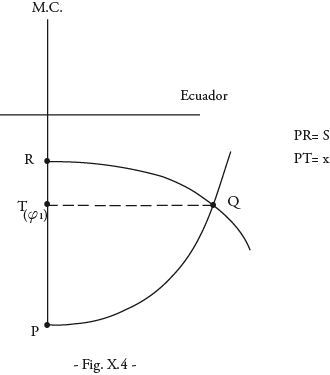
\includegraphics{repslatex-img82.png}

Para y=0 debe ser l=0; por lo tanto:

\[F\left(x\right)=q_1\] (X.24)

En la figura (X.4), S es el arco de meridiano del polo sur hasta la
latitud del punto Q; X es la coordenada Gauss, distancia del polo sur al
pie de la perpendicular desde Q al meridiano central, que se denomina T;
a la latitud del punto T se la denomina \(\varphi _1\). Por lo tanto
\(q_1\) se calcula en función de \(\varphi _1\).

Este valor puede ser obtenido en función de la coordenada X, en efecto
de la (VIII.13), arco de meridiano del polo sur a una altitud
cualquiera.

\[X=S=\alpha \cdot \varphi _1+\alpha \cdot {\frac{\pi }{2}}+\beta \cdot sen\left(2\cdot \varphi _1\right)+\gamma \cdot sen\left(4\cdot \varphi _1\right)+\delta \cdot sen\left(6\cdot \varphi _1\right)+\varepsilon \cdot sen\left(8\cdot \varphi _1\right)+\text{.}\text{.}\text{.}\]

El valor de \(\varphi_1\) se obtiene por aproximaciones sucesivas:

\[X=\alpha \cdot \left(\varphi _{1,1}+\frac{\pi }{2}\right)\]

\[\varphi _{1,1}=\frac{X}{\alpha }-\frac{\pi }{2}\]

Luego se introduce este primer valor de la latitud en la (VIII.13) para
obtener una segunda aproximación del valor de la latitud.

\[\varphi _{1,2}=\frac{1}{\alpha }\left(x-\alpha \cdot {\frac{\pi}{2}}-\beta \cdot sen\left(2\cdot \varphi _{1,1}\right)-\gamma \cdot sen\left(4\cdot \varphi _{1,1}\right)-\delta \cdot sen\left(6\cdot \varphi _{1,1}\right)-\varepsilon \cdot sen\left(8\cdot \varphi _{1,1}\right)\right)\]

\[\varphi _{1,2}=\left(\frac{x}{\alpha }-\frac{\pi}{2}\right)-\frac{\beta }{\alpha }\cdot sen\left(2\cdot \varphi _{1,1}\right)-\frac{\gamma }{\alpha }\cdot sen\left(4\cdot \varphi _{,\text{11}}\right)-\frac{\delta }{\alpha }\cdot sen\left(6\cdot \varphi _{1,1}\right)-\frac{\varepsilon }{\alpha }\cdot sen\left(8\cdot \varphi _{1,1}\right)\]

\[\varphi _{1,2}=\varphi _{1,1}-\frac{1}{\alpha }\left[\beta \cdot sen\left(2\cdot \varphi _{1,1}\right)-\gamma \cdot sen\left(4\cdot \varphi _{1,1}\right)-\delta \cdot sen\left(6\cdot \varphi _{1,1}\right)-\varepsilon \cdot sen\left(8\cdot \varphi _{1,1}\right)\right]\]

\[\varphi _{1,3}=\varphi _{1,1}-\left[\beta \cdot sen\left(2\cdot \varphi _{1,2}\right)+\gamma \cdot sen\left(4\cdot \varphi _{1,2}\right)+\delta \cdot sen\left(6\cdot \varphi _{1,2}\right)+\varepsilon \cdot sen\left(8\cdot \varphi _{1,2}\right)\right]\]

Se sigue iterando hasta que en la (VIII.13) introduciendo
\(\varphi_{1,j}\) dé como resultado el valor de X ingresado.

Para resolver las (X.23) se debe recordar:

\[dq=\frac{M\cdot d\varphi }{N\cdot \text{cos}\left(\varphi \right)}\]

Donde:

\[q=\int {\frac{M\cdot d\varphi }{N\cdot \text{cos}\left(\varphi \right)}}\]

Por lo tanto:

\[\varphi =f\left(q\right)=f\left[q_1+\left(q-q_1\right)\right]\]
Desarrollando en serie, tomando a \(\left(q-q_1\right)\) como
incremento, se tiene:

\[\varphi =\varphi _1+\frac{\mathit{d\varphi}}{dq}\left(q-q_1\right)+\frac{d^2\varphi}{dq^2}\left(q-q_1\right)^2+\text{.}\text{.}\text{.\]

Y por la (X.23) y (X.24) se tiene que:

\[\varphi =\varphi _1-\left[F^{II}\left(x\right)\frac{y^2}{2}-F^{IV}\left(x\right)\frac{y^4}{\text{24}}\right]\cdot {\frac{d\varphi }{dq}}\]

Para encontrar las expresiones se hallan las derivadas:

\[F^I\left(x\right)=\frac{dq}{dx}=\frac{dq}{\mathit{d\varphi}}\cdot {\frac{d\varphi }{dx}}\]

\[\frac{dq}{\mathit{d\varphi}}=\frac{M}{N\cdot \text{cos}\left(\varphi \right)}
\]\frac{d\varphi }{dx}=\frac{1}{M}\[

\]\frac{\mathit{d\varphi}}{dx}=\frac{1}{\text{cos}\left(\varphi \right)}\[

La segunda derivada se obtiene haciendo:

\]\frac{d^2q}{dx^2}=\frac{d}{\mathit{d\varphi}}\left(\frac{dq}{dx}\right)\frac{\mathit{d\varphi}}{dx}\[

Omitiendo el cálculo de
ésta y las derivadas de orden superior, como así también ciertas
transformaciones, se obtienen las siguientes expresiones:

\]l=\frac{y}{N_1\cdot \text{cos}\left(\varphi _1\right)}⋅
\left[1-\frac{y^2}{6\cdot N_1^2}\cdot \left(1+2\cdot t_1^2+n_1^2\right)+\frac{y^4}{\text{120}\cdot N_1^4}\cdot \left(5+\text{28}\cdot t_1^2+\text{24}\cdot t_1^4+6\cdot n_1^2+8\cdot n_1^2\cdot t_1^2\right)\right]\[

\]\emph{φ} =\emph{φ} \textsubscript{1}-\frac{y^2}{2\cdot N_1\cdot M_1}⋅
t\textsubscript{1}⋅
\left[1-\frac{y^2}{\text{12}\cdot N_1^2}\cdot \left(5+3\cdot t_1^2+n_1^2-9\cdot t_1^2\cdot n_1^2\right)+\frac{y^4}{\text{360}\cdot N_1^4}\cdot \left(\text{61}+\text{90}\cdot t_1^2+\text{45}\cdot t_1^4\right)\right]\[

Expresiones en las que el resultado se obtiene en radianes.

*** CONVERGENCIA DE MERIDIANOS.

[[file:repslatex-img83.png]]

Considerando la figura (X.5), NS representa la imagen del meridiano
que pasa por Q, WE el paralelo que pasa por el mismo punto, NC la
dirección paralela al meridiano central, es decir el norte de
cuadrícula.

El ángulo “c” formado por la tangente a NS en Q y la dirección NC, se
denomina convergencia de meridianos plana.

Considerando un punto Q1 infinitamente próximo, la diferencia de
coordenadas entre éste y Q es dx y dy. Del triángulo elemental de la
figura:

\]tg\left(c\right)=\frac{dx}{dy}\[
(X.26)

\]\frac{dx}{dy}\[

se halla de la ecuación de la curva WE, en la cual la latitud es
constante por tratarse de un paralelo y la (X.26) puede escribirse:

\]tg\left(c\right)=\frac{dx/dl}{dy/dl}\[
Las derivadas
\]\frac{dx}{dl}\[
y
\]\frac{dy}{dl}\[
se obtienen de diferenciar las expresiones de las coordenadas Gauss
(X.21.a) y (X.21.b), obteniéndose como primera aproximación:

\]\frac{dx}{dy}=l⋅ cos\textsuperscript{2}\left(\emph{φ} \right)⋅ N⋅ t\[
\]\frac{dy}{dl}=N⋅ cos\left(\emph{φ}
\right)\[ La convergencia de meridianos,
también como primera aproximación, será:

\]tg\left(c\right)=\frac{dx/dl}{dy/dl}=\frac{l\cdot
\text{cos}^2\left(\varphi \right)\cdot N\cdot t}{N\cdot
\text{cos}\left(\varphi \right)}=l⋅ sen\left(\emph{φ} \right)\[
\]tg\left(c\right)=l⋅ sen\left(\emph{φ} \right)\[ (X.27)

Con “l” en radianes.

Como resultado de la diferenciación de las expresiones de las
coordenadas Gauss con respecto a “l”, considerando todos los miembros y
la (X.27), se obtiene:

\]tg\left(c\right)=l⋅ sen\left(\emph{φ} \right)-\frac{l^3}{3}⋅
sen\left(\emph{φ} \right)⋅ cos\textsuperscript{2}\left(\emph{φ} \right)⋅
\left(1+t\textsuperscript{2}+3⋅
n\textsuperscript{2}+2n\textsuperscript{4}\right)+\frac{l^5}{\text{15}}⋅
sen\left(\emph{φ} \right)⋅ cos\textsuperscript{4}\left(\emph{φ} \right)⋅
\left(2+4⋅ t+2⋅ t\textsuperscript{4}\right)\[ Como

\]c=tg\left(c\right)-\frac{l^3}{3}⋅
tg\textsuperscript{3}\left(c\right)-\frac{l^5}{5}⋅
tg\textsuperscript{5}\left(c\right)\[
\]c=l⋅ sen\left(\emph{φ} \right)+\frac{l^3}{3}⋅ sen\left(\emph{φ}
\right)⋅ cos\textsuperscript{2}\left(\emph{φ} \right)⋅ \left(1+3⋅
n\textsuperscript{2}+2n\textsuperscript{4}\right)+\frac{l^5}{\text{15}}⋅
sen\left(\emph{φ} \right)⋅ cos\textsuperscript{4}\left(\emph{φ} \right)⋅
\left(2-t\textsuperscript{2}\right)\[
(X.28.a)

Si se desea la convergencia en función de las coordenadas planas, se
obtiene reemplazando “l” por las coordenadas rectangulares

\]d=\frac{y}{N_1}⋅ t\textsubscript{1}⋅ \left[1-\frac{y^2}{3\cdot
N_1^2}\cdot \left(1+t_1^2-n_1^2-2\cdot
n_1^4\right)+\frac{y^4}{N_1^4}\cdot
{\frac{\left(2+5\cdot t_1^2+3\cdot
t_1^4\right)}{\text{15}}}\right]\[ (X.28.b)

X.5.- MÓDULO DE DEFORMACIÓN.

Por tratarse de una proyección conforme, el módulo de deformación
lineal o factor de escala varía de acuerdo a las coordenadas pero una
vez fijadas, el módulo es el mismo en cualquier dirección.

De la (IX.2)

\]m\textsuperscript{2}=\frac{ds^2}{dS^2}=\frac{\left(dx\right)^2+\left(dy\right)^2}{\left(M\cdot
d\varphi \right)^2+\left(N\cdot \text{cos}\left(\varphi
\right)\cdot dl\right)^2}\[
\]m\textsuperscript{2}=\frac{\left(dy\right)^2\cdot
\left[1+\left(dx/dy\right)^2\right]}{\left(dl\right)^2\cdot
N^2\cdot \text{cos}^2\left(\varphi \right)\cdot
\left[1+\left(\frac{M\cdot d\varphi }{N\cdot
\text{cos}\left(\varphi \right)\cdot
dl}\right)^2\right]}\[

\]m\textsuperscript{2}=\left(\frac{dy}{dl}\right)\textsuperscript{2}\cdot
{\frac{1+\left(dx/dy\right)^2}{N^2\cdot
\text{cos}^2\left(\varphi \right)\cdot \left[1+\left(\frac{M\cdot
d\varphi }{N\cdot \text{cos}\left(\varphi \right)\cdot
dl}\right)^2\right]}}\[ Donde

\]1+\left(dx/dy\right)\textsuperscript{2}=1+tg\textsuperscript{2}\left(c\right)=sec\left(c\right)\[
Para el paralelo
\]d\emph{φ} /dl=0\[

\]m=\frac{dy}{dl}\cdot
{\frac{1}{N\cdot \text{cos}\left(\varphi \right)}}⋅
sec\left(c\right)\[ Calculando la derivada de “y” respecto de
“l” de la (X.21.b), sustituyendo el valor de “c”, se obtiene:

\]m=1+l\textsuperscript{2}⋅ cos\textsuperscript{2}\left(\emph{φ}
\right)⋅
\left(1+n\textsuperscript{2}\right)+\frac{l^4\cdot \text{cos}^4\left(\varphi
\right)}{\text{24}}⋅ \left(5-t\textsuperscript{2}+14⋅
n\textsuperscript{2}-28⋅ t\textsuperscript{2}⋅
n\textsuperscript{2}\right)\[ (X.29.a)

Expresión en la cual “l” se introduce en radianes.

Si se desea conocer la deformación lineal en función de las
coordenadas planas, se deduce:

\]m=1+\frac{y^2}{2\cdot R^2}+\frac{y^4}{\text{24}\cdot
R^4}\[ (X.29.b)

Donde:

\]R=\sqrt{M_1\cdot N_1}\[ X.6.- DEFORMACIONES LINEALES.

Cuando se desea conocer la deformación de una distancia finita,
tendiendo en cuenta que:

\]m=\frac{dl}{dL}\[
\]L=\overset{{l}}{\underset{{o}}{\int
}}{\frac{dl}{m}}\[ O bien:

\]l=\overset{{L}}{\underset{{o}}{\int }}{m\cdot dL}\[
Donde “L” es la distancia
sobre el elipsoide, “l” es la correspondiente en el plano y “m” es el
módulo de deformación lineal, por lo tanto:

\]L=\overset{{l}}{\underset{{o}}{\int }}{\left(1+\frac{y^2}{2\cdot
R^2}+\frac{y^4}{\text{24}\cdot
R^2}\right)}\textsuperscript{-1}dl\[ Se
desprecia el término de cuarto orden lo cual es aceptable hasta unos 3
grados del meridiano central.

\]L=\overset{{l}}{\underset{{o}}{\int }}{\left(1+\frac{y^2}{2\cdot
R^2}\right)}\textsuperscript{-1}dl\[ O bien
desarrollando el binomio:

\]L=\overset{{l}}{\underset{{o}}{\int }}{\left(1-\frac{y^2}{2\cdot
R^2}\right)}dl\[

[[file:repslatex-img84.png]]

Sea “p” en la figura (X.6) la distancia del elemento “dl” a partir de
“Q”, designando “y1” ordenada del punto Q y por “A” ángulo de dirección
o acimut de cuadrícula, se tiene que:

\]y=y\textsubscript{1}+p⋅ sen\left(A\right)\[
Por lo tanto:

\]L=\overset{{p=l}}{\underset{{p=o}}{\int
}}{\left(1-\frac{\left(y_1+p\cdot
sen\left(A\right)\right)^2}{2\cdot
R^2}\right)}dp\[

\]L=\overset{{p=l}}{\underset{{p=o}}{\int}}{\left(1-\frac{y_1^2+2\cdot y_1p\cdot sen\left(A\right)+p^2\cdot sen^2\left(A\right)}{2\cdot R^2}\right)}dp\[

\]L=p-\frac{y_1^2\cdot p}{2\cdot R^2}-\frac{2\cdot y_1\cdot p^2\cdot sen\left(A\right)}{2\cdot 2\cdot R^2}-\frac{p^3\cdot sen^2\left(A\right)}{6\cdot R^2}\textbar{}\textsubscript{0}\textsuperscript{l}\[

\]L=p⋅
\left[1-\frac{y_1^2}{2\cdot R^2}-\frac{y_1\cdot p\cdot sen\left(A\right)}{2\cdot R^2}-\frac{p^2\cdot sen^2\left(A\right)}{6\cdot R^2}\right]\textbar{}\textsubscript{0}\textsuperscript{l}\[

\]L=l⋅
\left[1-\frac{y_1^2}{2\cdot R^2}-\frac{y_1\cdot l\cdot sen\left(A\right)}{2\cdot R^2}-\frac{l^2\cdot sen^2\left(A\right)}{6\cdot R^2}\right]\[

Teniendo en cuenta que

\]\emph{Δ} y=y\textsubscript{2}-y\textsubscript{1}\[
\]\emph{Δ} y=l⋅ sen\left(A\right)\[

\]L=l⋅
\left[1-\frac{y_1^2}{2\cdot R^2}-\frac{y_1\cdot \left(y_2-y_1\right)}{2\cdot R^2}-\frac{\left(y_2-y_1\right)^2}{6\cdot R^2}\right]\[

Multiplicando y elevando al cuadrado el paréntesis y operando se llega:

\]L=l⋅
\left[1-\frac{\left(y_1^2+y_1\cdot y_2+y_2^2\right)}{6\cdot R^2}\right]\[

El módulo de deformación de una distancia finita será:

\]\frac{l}{L}=\left[1-\frac{\left(y_1^2+y_1\cdot y_2+y_2^2\right)}{6\cdot R^2}\right]\textsuperscript{-1}\[ O bien

\]\frac{l}{L}=1+\frac{\left(y_1^2+y_1\cdot
y_2+y_2^2\right)}{6\cdot R^2}\[ (X.30.a)

Donde:

\]R=\sqrt{M_1\cdot N_1}\[ ; ${\varphi =\frac{\varphi
_2+\varphi _1}{2}\]

En algunos casos es suficiente con tomar un valor promedio de la
coordenada ``y'', entonces:

\[y_m=\frac{y_2+y_1}{2}\] Reemplazando en (X.30.a)

\[\frac{l}{L}=1+\frac{y_m^2}{2\cdot R^2}\] (X.30.b)

X.7.- CORRECCIÓN ANGULAR.

En las proyecciones conformes los ángulos y las direcciones se trasladan
al elipsoide sin deformación pero la línea geodésica no queda
representada por una recta sino por alguna curva.

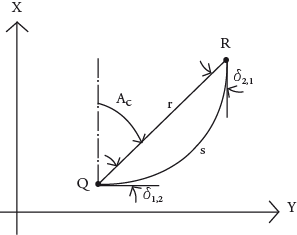
\includegraphics{repslatex-img85.png}

La conformidad se cumple en las tangentes a la curva que representa a la
línea geodésica. Si se mide un acimut en la carta respecto de la línea
recta que une los puntos del plano, se debe introducir una corrección
conocida como corrección del arco a la cuerda o corrección por curvatura
de la representación de la línea geodésica sobre un plano.

Se llega a la siguiente expresión suficientemente aproximada para
cualquier aplicación práctica:

\[\delta _{1,2}=\frac{\left(x_2-x_1\right)\cdot
\left(2\cdot y_1+y_2\right)}{6\cdot M\cdot N}\] (X.31.a)

\[\delta _{2,1}=\frac{\left(x_1-x_2\right)\cdot
\left(2\cdot y_2+y_1\right)}{6\cdot M\cdot N}\]

El resultado de la corrección viene expresado en radianes.

Tomando un valor promedio de la coordenada ``y'', se tiene:

\[\delta _{1,2}=\frac{\left(x_2-x_1\right)\cdot \left(3\cdot y_m\right)}{6\cdot M\cdot N\]
\[\delta _{1,2}=\frac{\Delta x\cdot y_m}{3\cdot
M\cdot N}\] (X.41.b)

Donde es inmediato que:

\[\delta _{1,2}=-\delta _{2,1}\] La distancia de la línea recta

que une los puntos debe ser corregida llamando a ésta ``r'' y a la
imagen de la línea geodésica ``s'' se tiene que:

\[dr=ds\cdot
\text{cos}\left(\delta \right)\] \$\{r=\overset{{s}}{\underset{{0}}{\int
}}{ds\cdot \text{cos}\left(\delta \right)}\[

\]dr=ds⋅ \left(1-\frac{\delta ^2}{2}\right)\[
\]dr-ds=-\left(\frac{\delta
^2}{2}\right)⋅ ds\[

La diferencia entre “r” y “s” es despreciable.

XI.1.- PROYECCIÓN TRANSVERSA DE MERCATOR. SISTEMA U.T.M.

El sistema U.T.M. (Universal Transverse Mercator) de la proyección de
Gauss fue recomendado por la Unión Geodésica y Geofísica Internacional
(IX Asamblea de Bruselas, 1951).

La proyección es cilíndrica transversal conforme; si es tangente al
elipsoide se trata de la proyección Gauss-Kruger y si es secante, del
sistema UTM.

Ambas proyecciones tienen mucho en común, sólo se diferencian en el
factor de escala, el ancho y numeración de las fajas y el origen de la
coordenada “x”.

XI.1.- ESPECIFICACIONES.

[[file:repslatex-img86.png]]

La proyección ordinaria es la de Gauss o transversa de Mercator. En la
proyección Trasversa Universal de Mercator, el cilindro envolvente sufre
una reducción y se torna secante cortando al elipsoide según dos líneas
AB y DE de la figura XI.1; la línea MC representa el meridiano. Los
círculos menores paralelos al meridiano central aparecen representados
en su verdadera magnitud, no así el meridiano central que aparecerá
representado con la misma longitud que los círculos menores, es decir se
reduce.

Sobre los círculos menores de sedancia el módulo de deformación o
factor de escala es igual a la unidad; en el meridiano central será un
valor menor que uno. Al módulo de deformación en el meridiano central se
lo denomina factor de reducción de escala.

En el sistema UTM el factor de escala en el meridiano central se
establece como:

\]k\textsubscript{0}=1-\frac{1}{\text{2500}}=0.9996\[ (XI.1)

Es decir, los valores de las distancias medidas sobre el meridiano
aparecen reducidas según ${k_0\].

Este factor de escala equivale a ubicar los círculos menores de sedancia
en una longitud de 1 37' 14'' a ambos lados del meridiano central. Sobre
esas líneas el factor de escala se hace igual a uno y más allá de ellas
supera este valor.

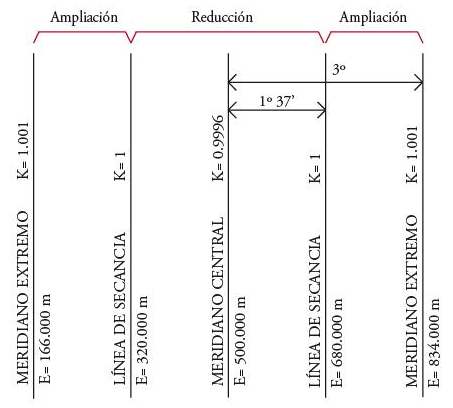
\includegraphics{repslatex-img87.png}

En la figura XI.2 se ilustra lo anterior. Existen dos zonas: una de
ampliación y otra de reducción.

En el sistema UTM los husos son de 6 de amplitud, 3 a cada lado del
meridiano central. La ampliación de la faja meridiana respecto de
Gauss-Kruger, se hace compatible con los módulos de deformación en los
extremos por haber introducido en el meridiano central el factor de
reducción \$\{k\textsubscript{0}\[.

Las líneas de tangencia se encuentran situadas a unos 180 km a ambos
lados del meridiano central, y los meridianos extremos a unos 334 km.

Las fajas de 6 de amplitud están limitados por los meridianos
múltiplos de 6 coincidiendo con los husos de la carta mundial al
millonésimo.

Cada sistema debe ser prolongado 30' sobre los contiguos, es decir los
puntos pertenecientes a cada faja tienen coordenadas en la propia y en
la contigua, creándose así una zona de superposición de 1 de ancho.

No son usadas las letras “X” e “Y” para designar las coordenadas, sino
“N” (norte) y “E” (este).

El origen de coordenadas planas en cada huso es el cruce del ecuador con
el meridiano central. La coordenada “N” se mide a partir del ecuador
pero para el hemisferio sur se las aumenta en 10.000.000 m evitando
valores negativos.

La coordenada “E” se mide a partir del meridiano central, positiva al
Este y negativa al Oeste. Para evitar valores negativos de “E” se
adjudica al meridiano central la coordenada 500.000 m.

El número de faja es el mismo que en la Carta Internacional al
millonésimo, ésto es de 1 a 60 a contar del antimeridiano de Greenwich.

El meridiano central de 177 (W) es la zona 1, el 171 (W) la zona 2 y así
cada 6.

La coordenada “E” para las líneas de sedancia son de acuerdo a lo
anterior son 680.000 m y 320.000 m al este y al oeste del meridiano
central respectivamente; y las coordenadas de los meridianos de borde de
faja son 834.000 m y 166.000 m al este y al oeste.

Las correspondencias entre los números de zona de las coordenadas UTM y
el número de fajas de proyección Gauss-Kruger en la República Argentina
de acuerdo a las convenciones adoptadas son:

\tablehead{}
|m3.457cm|m2.351cm|m3.448cm| Meridiano Central & Zona UTM &

Faja Gauss-Kruger -51 & 22 &

- -54 & &

7 -57 & 21 &

6 -60 & &

5 -63 & 20 &

4 -66 & &

3 -69 & 19 &

2 -72 & &

1 -75 & 18 &

-

En el sistema UTM el número de zona puede determinarse por medio de la
siguiente expresión:

\]ZONA=\frac{\left(\text{183}+\lambda
_0\right)}{6}\[(XI.2)

Donde ${\lambda _0\] es la longitud del meridiano central y se debe
introducir con su signo.

El número de faja de la proyección Gauss-Kruger para el territorio
argentino se puede encontrar por medio de:

\[FAJA=\frac{\left(\text{75}+\lambda
_0\right)}{3}\] (XI.3)

XI.2.- TRANSFORMACIÓN DE COORDENADAS GEOGRÁFICAS EN PLANAS.

El planteo de las expresiones de las coordenadas UTM es similar al de
las Gauss-Kruger, y es a través de las funciones de variable compleja:

\[x+iy=f\left(q+il\right)\] (XI.4)

Considerando puntos en el meridiano central

\[x=f\left(q\right)=B\] Donde ``B'' es el arco de meridiano elipsóidico
que va del ecuador hasta la latitud considerada como se determinó en la
expresión (VIII.12).

Se desarrolla en serie de Taylor tomando ``l'' como incremento de la
misma forma que en la proyección Gauss-Kruger determinándose expresiones
similares con la diferencia que en el meridiano central se cuentan las
coordenadas a partir del ecuador.

Pero para reducir las deformaciones y poder ampliar las zonas, se afectó
al meridiano central según un factor de reducción
\$\{k\textsubscript{0}\[, de
manera tal que las distancias sobre el meridiano central aparecen
reducidas por el factor de escala, es decir que el arco de meridiano del
ecuador a la latitud en consideración habrá que afectarlo por este
factor

\]f\left(q\right)=k\textsubscript{0}⋅ B\[ (XI.5)

la imagen geométrica de la proyección con este artificio del factor de
escala, se obtiene considerando un cilindro secante en lugar de tangente
según dos líneas que se representan en su verdadera magnitud. En lugar
de una línea sin deformación se obtienen dos, simétricas respecto del
meridiano central.

Las expresiones de las coordenadas UTM son similares a las de Gauss
con las siguientes modificaciones:

\]N=k\textsubscript{0}\cdot [B+\frac{l^2\cdot \text{cos}^2\left(\varphi \right)\cdot N\cdot t}{2}+\frac{l^4\cdot \text{cos}^4\left(\varphi \right)\cdot N\cdot t\cdot \left(5-t^2+9\cdot n^2+4\cdot n^4\right)}{\text{24}}+$$

$$+{\frac{l^6\cdot \text{cos}^6\left(\varphi \right)\cdot N\cdot t\cdot \left(\text{61}-\text{58}\cdot t^2+t^4+\text{270}\cdot n^2-\text{330}\cdot t^2\cdot n^2\right)}{\text{720}}}]\[

\]E=500.000+k\textsubscript{0}\cdot [l\cdot \text{cos}\left(\varphi \right)\cdot N+\frac{l^3\cdot \text{cos}^3\left(\varphi \right)\cdot N\cdot t\cdot \left(1-t^2+n^2\right)}{6}+$$

$+{\frac{l^5\cdot \text{cos}^5\left(\varphi \right)\cdot N\cdot t\cdot \left(5-\text{18}\cdot t^2+t^4+\text{14}\cdot n^2-\text{58}\cdot t^2\cdot n^2\right)}{\text{120}}}]\[

En el hemisferio sur se le suma la cantidad de 10.000.000 m a la
coordenada “N”.

En el problema recíproco, es decir la transformación de coordenadas
planas a geográficas se computarán con las mismas expresiones que las de
Gauss-Kruger con la diferencia de que el valor de “y” se tomará como:

\]y=\frac{\left(E-\text{500}\text{.}\text{000}\right)}{k_0}\[
(XI.7)

Este mismo valor de “y” se adoptará para el círculo de la convergencia
meridiana en la expresión (X.28.b).

El módulo de deformación lineal se calculará introduciendo el valor de
\]k\textsubscript{0}\[:

\]m=k\textsubscript{0}⋅ \left(1+\frac{y^2}{2\cdot
R^2}+\frac{y^4}{\text{24}\cdot R^4}\right)\[ (XI.8)

En cuanto a la deformación de distintas finitas la consideración es la
misma de modo que:

\]\frac{l}{L}=k\textsubscript{0}⋅ \left(1+\frac{y_1^2+y^1\cdot
y^2+y_2^2}{6\cdot R^2}\right)\[ (XI.9)

La corrección el arco a la cuerda se obtiene de las (X.41.a) o
(X.41.b) pero teniendo en cuenta la (XI.7) en las (XI.8) y (XI.9);
también se introduce el valor de “y” de la (XI.7).

XI.3.- UNA EXPRESIÓN PARA AMBAS PROYECCIONES.

En las siguientes expresiones se debe tener en cuenta el signo de la
latitud y longitud, y son válidas para el hemisferio sur.

\]X=Q+k\textsubscript{0}\cdot [B+\frac{l^2\cdot \text{cos}^2\left(\varphi \right)\cdot N\cdot t}{2}+\frac{l^4\cdot \text{cos}^4\left(\varphi \right)\cdot N\cdot t\cdot \left(5-t^2+9\cdot n^2+4\cdot n^4\right)}{\text{24}}+$$

$$+{\frac{l^6\cdot \text{cos}^6\left(\varphi \right)\cdot N\cdot t\cdot \left(\text{61}-\text{58}\cdot t^2+t^4+\text{270}\cdot n^2-\text{330}\cdot t^2\cdot n^2\right)}{\text{720}}}]\[

\]Y=F+500.000+k\textsubscript{0}\cdot [l\cdot \text{cos}\left(\varphi \right)\cdot N+\frac{l^3\cdot \text{cos}^3\left(\varphi \right)\cdot N\cdot t\cdot \left(1-t^2+n^2\right)}{6}+$$

$$+{\frac{l^5\cdot \text{cos}^5\left(\varphi \right)\cdot N\cdot t\cdot \left(5-\text{18}\cdot t^2+t^4+\text{14}\cdot n^2-\text{58}\cdot t^2\cdot n^2\right)}{\text{120}}}]\[

Donde:

\]t=tg\left(\emph{φ} \right)\[
\]n\textsuperscript{2}=e'\textsuperscript{2}⋅
cos\textsuperscript{2}\left(\emph{φ} \right)\[
\]e'\textsuperscript{2}=\frac{a^2-b^2}{b^2}\[
\]N=\frac{a}{\left[1-e^2\cdot
sen^2\left(\varphi
\right)\right]^{1/2}}\[ \]l=\emph{λ} -\emph{λ}
\textsubscript{0}\[ (expresada
en radianes)

\]\emph{λ}
\textsubscript{0}\[ es la longitud del meridiano central de la faja
Gauss-Kruger o zona UTM en la que se proyectan los puntos.

“B” es el arco de meridiano desde el ecuador hasta la latitud
considerada, por la expresión (VIII.12).

\]B=\emph{α} ⋅ \emph{φ} +\emph{β} ⋅ sen\left(2⋅ \emph{φ}
\right)+\emph{γ} ⋅ sen\left(4⋅ \emph{φ} \right)+\emph{δ} ⋅ sen\left(6⋅
\emph{φ} \right)+\emph{ε} ⋅ sen\left(8⋅ \emph{φ} \right)\[
En el caso de Gauss-Kruger la coordenada por el meridiano central se
mide a partir del polo sur; para que ésto se cumpla en la expresión
(XI.10.a) se hace:

\]Q=\frac{a\cdot \pi }{2}\[ En el caso de coordenadas UTM para el
hemisferio sur, por lo anteriormente visto, se tiene que:

\]Q=10.000.000m\[ El factor de
escala:

\]k\textsubscript{0}=1\[(Gauss-Kruger)

\]k\textsubscript{0}=0.9996\[(U.T.M.)

“F” se refiere al número de faja, introducido en los millones de la
coordenada “Y”

\]F=\left[\frac{\left(\text{75}+\lambda
_0\right)}{3}\right]⋅ 10\textsuperscript{6}\[(Gauss-Kruger)

\]F=0\[(U.T.M.)

En la proyección UTM debe agregarse como información el valor de la
zona, ésto es:

\]ZONA=\frac{\text{183}+\lambda _0}{6}\[
En la proyección Gauss-Kruger, los resultados de las coordenadas
(XI.10.a) y (XI.10.b) se expresan como “X” e “Y”. En el sistema UTM como
“N” en lugar de “X”, y “E” en lugar de “Y”.

En ambas proyecciones, para la transformación son necesarias como
datos la latitud y longitud de los puntos con cuatro decimales, los
parámetros del elipsoide de referencia, longitud del meridiano central.

En la transformación de coordenadas planas en coordenadas geográficas
se puede escribir:

\]\emph{φ} =\emph{φ} \textsubscript{1}-\frac{y^2}{2\cdot M_1\cdot
N_1}⋅ t\textsubscript{1}⋅ \left[1-\frac{y^2}{\text{12}\cdot
N_1^2}\cdot \left(5+3\cdot t_1^2+n_1^2-9\cdot
t_1^2\cdot n_1^2\right)+\frac{y^4}{\text{360}\cdot
N_1^4}\cdot \left(\text{61}+\text{90}\cdot
t_1^2+\text{45}\cdot t_1^4\right)\right]\[ (XI.11.a)

\]\emph{λ} =\emph{λ}
\textsubscript{0}+\frac{y}{N_1\cdot \text{cos}\left(\varphi
_1\right)}⋅ \left[1-\frac{y^2}{6\cdot N_1^2}\cdot
\left(1+2\cdot
t_1^2+n_1^2\right)+\frac{y^4}{\text{120}\cdot
N_1^4}\cdot \left(5+\text{28}\cdot t_1^2+\text{24}\cdot
t_1^4+6\cdot n_1^2-8\cdot n_1^2\cdot
t_1^2\right)\right]\[ (XI.11.b)

Donde:

\]M=\frac{a\cdot \left(1-e^2\right)}{\left[1-e^2\cdot sen^2\left(\varphi \right)\right]^{3/2}}\[
\]y=\frac{\left(Y-F-\text{500}\text{.}\text{000}\right)}{k_0}\[
\]NF=\frac{F}{\text{10}^6}\[
(número de faja en Gauss-Kruger)

\]\emph{λ} \textsubscript{0}=3⋅ NF-75\[(para
Gauss-Kruger)

\]\emph{λ} \textsubscript{0}=6⋅ ZONA-183\[(para UTM)

es el arco de meridiano correspondiente a “x” siendo:

\]x=\frac{X-Q}{k_0}\[
\]Q=\frac{\alpha \cdot \pi }{2}\[(para Gauss-Kruger)

\]Q=10.000.000m\[(para UTM)

El valor de ${\varphi _1\] se halla con las aproximaciones sucesivas
vistas en (X.3).

Los resultados de las (XI.11) están expresados en radianes; notar que
tanto \[\varphi _1\] y \[\lambda _0\] deben ser introducidos en
radianes.

Para la transformación son necesarias como dato X o N, Y o E, los
parámetros del elipsoide de referencia.

\end{document}
